
\excercise{DemoTask und UI}

\begin{enumerate}
    \item[a)] Nun wollen wir wieder ein Spiel starten. Diesesmal mit einem Task:
    
    \begin{lstlisting}
    Game myGame = new Game("Hello World", new DemoTask());
    \end{lstlisting}
    
    Nun wollen wir das Spiel (Game) auch starten können. Also führen wir die Operation .run() darauf aus. 
    
    \begin{lstlisting}
    myGame.run();
    \end{lstlisting}
    
    Starte das Spiel mit dem kleinen Play-Button oben in der Werkzeugleiste und schau dich ein wenig im Fenster um das aufgeht.
    
    \item[b)] Nun erweitern wir das Game-Objekt um ein Parameter. Füge einen DemoTaskVerifier Objekt hinter dem DemoTask-Objekt hinzu. Was verändert sich im Spiel? Versuche den Task zu erfüllen.
    
    \begin{lstlisting}
    Game myGame = new Game("Hello World", new DemoTask(), new DemoTaskVerifier());
    \end{lstlisting}
    
    \end{enumerate}
    \begin{Infobox}[Der Refresh Button]
    Wichtig: Wenn ihr überprüfen wollt ob ihr eure Aufgabe erledigt habt, müsst ihr auf \fbox{Task Status} und dann auf \fbox{Refresh} klicken.
    \end{Infobox}
    \begin{enumerate}
    
    \item[c)] Finde sowohl im Spiel als auch in Eclipse die Konsole. das ist ein Feld in dem Text ausgegeben wird:
    \begin{center}
        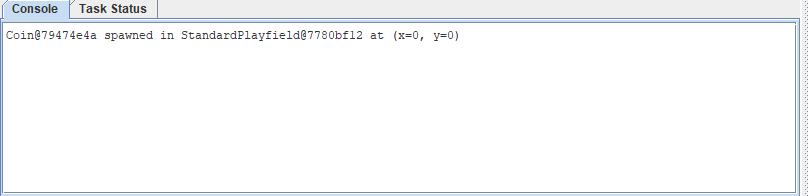
\includegraphics[width=\linewidth]{./figures/console.PNG}
    \end{center}
    
    Was denkst du bedeutet der Text der ausgegeben wird?
    
    \item[d)] Nun suche nach der Stelle im Code in dem die erste Münze erzeugt wird. Kleiner Tipp: Verwende dafür \fbox{Strg} um auf Objekte zu klicken und in ihre Klasse zu kommen.
\end{enumerate}
